\documentclass{iopjournal}

\usepackage{amsmath,amssymb}
\usepackage{graphicx}
\usepackage{booktabs}
\usepackage{hyperref}
\usepackage{multirow}

\begin{document}

\articletype{Paper}

\title{Riemannian Filter Bank Tangent Space Features for EEG-Based Vigilance Estimation with Multimodal Fusion}

\author{Xiangzhu Li$^{1}$\orcid{0009-0002-4157-6201}, Huang Tan$^{2}$\orcid{0009-0002-7101-6731} and Li Zhang$^{1,*}$\orcid{0000-0000-0000-0000}\textsuperscript{\textbf{[TO FILL]}}}

\affil{$^1$Shenzhen Hospital of Integrated Traditional Chinese and Western Medicine, Guangzhou University of Chinese Medicine, Shenzhen 518104, China}
\affil{$^2$University of Electronic Science and Technology of China, Chengdu 611731, China}
\affil{$^*$Author to whom any correspondence should be addressed.}

\email{lxz142537@163.com (XL), tanhuang@std.uestc.edu.cn (HT), thyysjwk1bq@163.com (LZ)}

\keywords{EEG, vigilance estimation, Riemannian geometry, filter bank tangent space, multimodal fusion, SEED-VIG}

\begin{abstract}

\textbf{Objective.} Differential entropy (DE) features, the standard for EEG-based vigilance estimation, capture per-channel spectral energy but discard the inter-channel covariance structure that reflects the coordinated neural dynamics of drowsiness transitions. We present the first systematic evaluation of Riemannian filter bank tangent space (FBTS) features for continuous EEG vigilance regression.

\textbf{Approach.} The FBTS pipeline bandpass-filters EEG epochs into five frequency bands, computes regularized SPD covariance matrices, projects them onto the Riemannian tangent space under the affine-invariant metric, and feeds the concatenated features to SVR. On the SEED-VIG dataset (23 subjects, 17-channel EEG + forehead EOG), we conduct within-subject 5-fold cross-validation, leave-one-subject-out (LOSO) generalization, and cross-dataset transfer to SEED emotion recognition, with comprehensive ablation across channel subsets, frequency-band partitions, Riemannian metrics, and multimodal fusion strategies.

\textbf{Main results.} Single-modality FBTS matches DE (COR 0.520 vs.\ 0.521; $p=0.984$). Under EEG+EOG fusion, FBTS significantly outperforms DE (COR 0.618 vs.\ 0.586; $t(22)=2.13$, $p=0.044$, $d=0.45$). LOSO reveals the strongest result: FBTS+EOG with only 6 temporal channels achieves COR 0.835---a 34\% improvement over within-subject DE. A 4-channel forehead variant retains 99\% of full-channel performance (COR 0.613). Cross-dataset validation on SEED yields 86.1\% emotion classification accuracy.

\textbf{Significance.} FBTS emerges as a general-purpose EEG feature extractor---originally developed for motor imagery classification, now validated for vigilance regression, cross-subject transfer, and cross-task generalization---with particular strength in multimodal fusion and wearable scenarios.

\end{abstract}

% =================================================================
\section{Introduction}

Vigilance---the ability to maintain sustained attention over prolonged periods---is a critical cognitive state whose degradation underlies numerous safety-critical failures, from traffic accidents caused by driver fatigue~\cite{zheng2017multimodal} to lapses in air traffic control and medical errors during extended clinical shifts~\cite{barger2006impact}. Electroencephalography (EEG) provides a direct, high-temporal-resolution window into brain dynamics and has emerged as the modality of choice for objective vigilance monitoring~\cite{shi2013differential, lin2014wireless}.

\subsection{Clinical significance of vigilance monitoring}

The clinical and public health importance of objective vigilance assessment extends across multiple domains. Drowsy driving accounts for approximately 20\% of fatal motor vehicle accidents worldwide, with an estimated 100,000 police-reported crashes annually in the United States alone attributable to driver fatigue~\cite{lyznicki1998sleepiness}. Beyond transportation safety, vigilance deficits are a hallmark symptom of numerous neurological and psychiatric conditions including obstructive sleep apnea (OSA), narcolepsy, attention-deficit/hyperactivity disorder (ADHD), traumatic brain injury, and shift work sleep disorder~\cite{zhang2022eegbased,rosenberg2016neuromarker}. In clinical settings, the current gold standard for objective sleepiness assessment---the Multiple Sleep Latency Test (MSLT)---requires polysomnography in a dedicated sleep laboratory, is costly, time-consuming, and provides only episodic snapshots rather than continuous monitoring~\cite{littner2005practice}. A reliable EEG-based continuous vigilance estimator could enable ambulatory monitoring in naturalistic environments, offering an accessible complement to laboratory-based assessments~\cite{kaiser2022wearable}.

From a neurophysiological perspective, the transition from alert wakefulness to drowsiness involves a well-characterized sequence of EEG changes: increased power in theta (4--8\,Hz) and alpha (8--13\,Hz) bands, particularly over posterior and central regions, accompanied by decreased beta (13--30\,Hz) and gamma ($>$30\,Hz) activity~\cite{olbrich2009eeg, jagannathan2019tracking}. These spectral shifts reflect progressive disengagement of thalamocortical arousal circuits and the ascending reticular activating system (ARAS), with functional magnetic resonance imaging (fMRI) studies confirming reduced connectivity between the thalamus and prefrontal cortex during drowsiness~\cite{tagliazucchi2014large}. Importantly, these changes are not uniform across cortical regions: posterior-to-anterior shifts in alpha topography and inter-hemispheric coherence changes have been documented~\cite{strijkstra2003subjective}, suggesting that \emph{inter-channel relationships}---covariance and connectivity patterns---carry vigilance-relevant information beyond what per-channel spectral power alone can capture.

The standard approach to EEG-based vigilance estimation consists of two stages: (1) extraction of spectral features such as power spectral density (PSD) or differential entropy (DE) from predefined frequency bands, and (2) regression using support vector regression (SVR) or related models~\cite{zheng2017multimodal, huo2016driving}. DE features, which approximate the logarithm of the signal variance under a Gaussian assumption, have consistently outperformed PSD across multiple EEG paradigms including emotion recognition and vigilance estimation~\cite{duan2013differential, shi2013differential}.

However, spectral features operate independently on each EEG channel: the DE of channel $i$ in band $j$ is computed without reference to channel $k \neq i$. This deliberately discards the covariance structure between channels---information that reflects the functional connectivity and coordinated neural dynamics that characterize transitions between alert and drowsy states.

\subsection{Riemannian geometry for EEG}

In the motor imagery brain-computer interface (BCI) literature, a fundamentally different feature paradigm has achieved state-of-the-art performance: representing EEG epochs as symmetric positive definite (SPD) covariance matrices and applying Riemannian geometry to classify them~\cite{congedo2017riemannian, barachant2012multiclass}. The filter bank tangent space (FBTS) pipeline---bandpass filtering into multiple frequency bands, computing SPD covariance matrices per band, projecting onto the tangent space of the Riemannian manifold, and concatenating the resulting vectors---has proven robust across subjects and recording conditions~\cite{barachant2012multiclass}.

Despite this success in discrete classification tasks, and recent extensions to deep SPD network learning for EEG decoding~\cite{huang2022spd, xu2023riemannian}, Riemannian tangent space features have \emph{never} been systematically evaluated for \emph{continuous regression} in vigilance estimation. This gap is notable for two reasons. First, vigilance estimation is a regression problem (predicting a continuous PERCLOS score from 0 to 1), and it is not obvious that features optimized for discrete class separation will transfer to a continuous target. Second, the channel covariance structure that Riemannian features preserve may be especially informative for vigilance, where transitions between alertness and drowsiness involve coordinated spectral changes across multiple brain regions~\cite{zheng2017multimodal}.

\subsection{Contributions}

This paper makes the following contributions:

\begin{enumerate}
  \item We present the first systematic evaluation of Riemannian filter bank tangent space (FBTS) features for continuous EEG-based vigilance estimation, adapting the pipeline from discrete classification to SVR-based regression.
  \item Through comprehensive experiments on the SEED-VIG dataset (23 subjects, 17-channel EEG + forehead EOG, 885 epochs/subject), we compare FBTS against DE and PSD baselines in both single-modality and EEG+EOG fusion settings.
  \item We demonstrate that while single-modality FBTS and DE perform equivalently (COR 0.520 vs.\ 0.521; $t(22)=-0.02$, $p=0.984$), FBTS+EOG fusion significantly outperforms DE+EOG (COR 0.618 vs.\ 0.586; $t(22)=2.13$, $p=0.044$, Cohen's $d=0.45$).
  \item We show that the channel-agnostic nature of FBTS enables a lightweight 4-channel forehead variant (COR 0.613) that retains 99\% of full-channel performance, supporting wearable deployment.
  \item Through leave-one-subject-out (LOSO) evaluation, we reveal FBTS's cross-subject advantage: FBTS+EOG with only 6 temporal channels achieves COR 0.835---the strongest result in this study and a 34\% improvement over within-subject DE performance---demonstrating that Riemannian geometry plus ocular fusion yields exceptional cross-subject generalization.
  \item We validate FBTS across datasets and tasks: the same pipeline achieves 86.1\% three-class emotion classification accuracy on SEED, confirming its general-purpose EEG feature extraction capability.
\end{enumerate}

% =================================================================
\section{Methods}

\subsection{Filter Bank Tangent Space Regression}

\subsubsection{Neurophysiological rationale}

The choice of FBTS features for vigilance estimation is motivated by the neurophysiology of drowsiness transitions. As alertness decreases, the brain undergoes a systematic reorganization of functional connectivity: thalamocortical relay nuclei disengage from prefrontal control~\cite{tagliazucchi2014large}, posterior alpha generators shift anteriorly~\cite{strijkstra2003subjective}, and inter-hemispheric coherence in the default mode network increases~\cite{olbrich2009eeg}. These connectivity-level changes are poorly captured by per-channel spectral features such as DE or PSD, which treat each electrode as an independent information source. In contrast, the SPD covariance matrix $\mathbf{\Sigma}_b \in \mathbb{R}^{C \times C}$ for frequency band $b$ encodes the pairwise linear interactions between all $C$ EEG channels, providing a compact representation of the instantaneous functional connectivity structure. The Riemannian tangent space projection then maps these matrices into a Euclidean vector space while preserving the geometric relationships of the underlying SPD manifold, enabling standard regression models to operate on connectivity-informed features. This approach aligns with a growing clinical literature demonstrating that vigilance states are more accurately decoded from functional connectivity measures than from regional spectral power alone~\cite{tagliazucchi2014large, jagannathan2019tracking}.

The OAS shrinkage estimator~\cite{chen2010shrinkage} used in our covariance estimation step is particularly relevant for EEG data: it provides a well-conditioned estimate even when the number of time samples per epoch ($T=1600$ at 200\,Hz for 8\,s epochs) is modest relative to the channel dimensionality, a common scenario in clinical EEG with dense electrode montages.

\subsubsection{Pipeline description}

The FBTS pipeline, originally developed for motor imagery classification~\cite{barachant2012multiclass}, is adapted here for continuous regression. Given an EEG epoch $\mathbf{X} \in \mathbb{R}^{C \times T}$ with $C$ channels and $T$ time samples, the pipeline proceeds as follows:

\noindent\textbf{Step 1: Filter Bank.} The epoch is bandpass-filtered (4th-order Butterworth, zero-phase) into $B$ frequency bands $\{ (f^\ell_b, f^h_b) \}_{b=1}^B$. We use $B=5$ bands: delta (1--4\,Hz), theta (4--8\,Hz), alpha (8--14\,Hz), beta (14--31\,Hz), and gamma (31--50\,Hz), matching the frequency decomposition used for DE features in the SEED-VIG literature~\cite{zheng2017multimodal}.

\noindent\textbf{Step 2: Covariance Estimation.} For each band $b$, the $C \times C$ sample covariance matrix is computed:
\begin{equation}
  \mathbf{\Sigma}_b = \frac{1}{T-1} \tilde{\mathbf{X}}_b \tilde{\mathbf{X}}_b^\top \in \mathbb{R}^{C \times C},
\end{equation}
where $\tilde{\mathbf{X}}_b$ is the bandpass-filtered and mean-centered epoch. We apply Oracle Approximating Shrinkage (OAS) regularization~\cite{chen2010shrinkage} for numerical stability. Each $\mathbf{\Sigma}_b$ lies on the manifold $\mathcal{S}_{C}^{++}$ of $C \times C$ SPD matrices.

\noindent\textbf{Step 3: Tangent Space Projection.} The Riemannian mean $\bar{\mathbf{\Sigma}}_b$ of the training covariance matrices is computed under the affine-invariant metric. Each matrix is then projected onto the tangent space at $\bar{\mathbf{\Sigma}}_b$ via the logarithmic map:
\begin{equation}
  \mathbf{s}_b = \mathrm{upper}\left( \bar{\mathbf{\Sigma}}_b^{-1/2} \; \log\left( \bar{\mathbf{\Sigma}}_b^{-1/2} \mathbf{\Sigma}_b \bar{\mathbf{\Sigma}}_b^{-1/2} \right) \; \bar{\mathbf{\Sigma}}_b^{1/2} \right),
\end{equation}
yielding a vector $\mathbf{s}_b \in \mathbb{R}^{C(C+1)/2}$ of tangent space features per band.

\noindent\textbf{Step 4: Feature Selection and Regression.} The tangent space vectors from all $B$ bands are concatenated into $\mathbf{f} = [\mathbf{s}_1; \ldots; \mathbf{s}_B] \in \mathbb{R}^{B \cdot C(C+1)/2}$. Univariate feature selection ($F$-test) retains the top $K=100$ features most correlated with vigilance. A support vector regression model with radial basis function kernel ($C=1.0$, $\gamma=\text{scale}$) predicts the continuous PERCLOS score. A 3-point moving average filter is applied to the prediction sequence for temporal smoothing.

\subsection{Baseline Features}

\noindent\textbf{Differential Entropy (DE).} DE for channel $i$ in frequency band $b$ is computed as
\begin{equation}
  h_{i,b} = \frac{1}{2} \log (2\pi e \sigma_{i,b}^2),
\end{equation}
where $\sigma_{i,b}^2$ is the signal variance in band $b$. DE features are extracted using pre-computed features from SEED-VIG (short-time Fourier transform, 8\,s non-overlapping Hamming window, LDS smoothing). For 17 channels and 5 bands, this yields a 85-dimensional vector per epoch.

\noindent\textbf{Power Spectral Density (PSD).} PSD features are extracted identically to DE but without the logarithmic transformation, directly using the band-limited signal power.

\noindent\textbf{EOG Features.} The SEED-VIG dataset includes 36-dimensional forehead EOG features extracted via wavelet-based blink and saccade detection~\cite{zheng2017multimodal}. We use the ICA-separated variant as the primary EOG representation.

\subsection{Multimodal Fusion}

Feature-level fusion is used throughout: feature vectors from different modalities are concatenated before feature selection and regression. All features are standardized ($z$-score) per training fold.

\subsection{Evaluation Protocol}

Following the standard SEED-VIG protocol~\cite{zheng2017multimodal}, each subject's 885 epochs are divided into five chronological segments of 177 epochs each. Four segments train the model; the remaining segment is held out for testing. Performance is measured by Pearson correlation coefficient (COR) and root mean square error (RMSE). Global COR is computed by concatenating predictions across all five folds. Statistical significance is assessed using paired two-tailed $t$-tests ($\alpha = 0.05$) across the 23 subjects.

% =================================================================
\section{Experiments}
\label{sec:experiments}

All experiments were performed on a Linux workstation (Dell PowerEdge R750, Intel Xeon, 64 GB RAM) with Python 3.11. Results are reproducible from the unified execution script \texttt{run\_all.py}, with statistical tests recomputed on the full 23-subject SEED-VIG dataset using paired two-tailed $t$-tests and Cohen's $d$ effect size. Experiment configurations span the complete matrix described in the project documentation (SKILL.md \S3).

\subsection{Dataset}

SEED-VIG~\cite{zheng2017multimodal} contains EEG and EOG recordings from 23 subjects (mean age 23.3, 12 females) performing a monotonous simulated driving task for approximately two hours. The experimental procedures involving human participants were approved by the Ethics Committee of Shanghai Jiao Tong University, and written informed consent was obtained from all participants prior to the experiments~\cite{zheng2017multimodal}. All data were anonymized before release. EEG was recorded from 17 channels at 200\,Hz: six temporal channels (FT7, FT8, T7, T8, TP7, TP8) and eleven posterior channels (CP1, CP2, P1, PZ, P2, PO3, POZ, PO4, O1, OZ, O2; CPZ excluded for proximity to reference). Forehead EOG was simultaneously recorded from seven electrodes. Vigilance was annotated using PERCLOS (percentage of eye closure) computed from SMI eye-tracking glasses, yielding a continuous score in $[0,1]$. Data were segmented into 885 non-overlapping 8-second epochs per subject.

\subsection{Experimental Configurations}

We evaluate the following feature configurations, all with SVR regression:

\begin{itemize}
  \item \textbf{Single-modality:} DE (17ch, 6ch temporal), PSD (17ch, 6ch temporal), FBTS-Riemannian (17ch, 6ch temporal, 4ch forehead; 5-band and 8-band variants).
  \item \textbf{EEG+EOG fusion:} DE+EOG, FBTS+EOG (all channel variants).
  \item \textbf{EEG+EEG fusion:} DE+FBTS (complementary feature spaces).
  \item \textbf{Three-modal fusion:} DE+FBTS+EOG.
\end{itemize}

The 8-band variant subdivides alpha (8--10, 10--12, 12--14\,Hz) and beta (14--20, 20--30\,Hz) for finer spectral resolution. The 4-channel ``forehead'' variant uses FT7, FT8, T7, and T8.

\begin{table}
\caption{Single-modality feature comparison (23 subjects, 5-fold cross-validation). DE and FBTS achieve equivalent performance; both significantly outperform PSD. FBTS benefits more from additional channels (17ch) than from additional frequency bands (8-band vs.\ 5-band).}
\centering
\begin{tabular}{lcccccc}
\toprule
\textbf{Feature} & \textbf{Channels} & \textbf{Bands} & \textbf{COR} & \textbf{RMSE} & \textbf{Global COR} & \textbf{Dim} \\
\midrule
DE (LDS)     & 17 & 5 & 0.521 $\pm$ 0.180 & 0.140 & 0.664 & 85 \\
FBTS (Riem.) & 17 & 5 & 0.520 $\pm$ 0.167 & 0.139 & 0.660 & 765 \\
FBTS (Riem.) & 17 & 8 & 0.520 $\pm$ 0.167 & 0.138 & 0.661 & 1224 \\
FBTS (Riem.) & 6 (temp.) & 5 & 0.508 $\pm$ 0.172 & 0.144 & 0.639 & 105 \\
DE (LDS)     & 6 (temp.) & 5 & 0.491 $\pm$ 0.179 & 0.146 & 0.627 & 30 \\
PSD (LDS)    & 17 & 5 & 0.489 $\pm$ 0.168 & 0.153 & 0.600 & 85 \\
FBTS (Riem.) & 4 (fore.) & 5 & 0.490 $\pm$ 0.179 & 0.142 & 0.629 & 50 \\
PSD (LDS)    & 6 (temp.) & 5 & 0.474 $\pm$ 0.168 & 0.160 & 0.568 & 30 \\
\bottomrule
\end{tabular}
\label{tab:single}
\end{table}

\subsection{Single-Modality Results}

Table~\ref{tab:single} presents single-modality results. Three observations are salient. First, FBTS and DE achieve \emph{statistically equivalent} performance (DE: 0.521, FBTS-5band: 0.520; $t(22)=-0.02$, $p=0.984$). This is a meaningful null result: Riemannian tangent space features, which capture a fundamentally different signal property (inter-channel covariance structure) than DE (per-channel spectral energy), yield comparable single-modality regression accuracy. Second, both DE and FBTS significantly outperform PSD ($p < 0.01$ for all comparisons), confirming previous findings that entropy-based features are superior to raw spectral power for EEG state estimation~\cite{shi2013differential}. Third, FBTS benefits more from additional channels than DE does: DE drops from 0.521 (17ch) to 0.491 (6ch), a 5.8\% relative decrease, while FBTS drops from 0.520 to 0.508, only 2.3\%. The full-channel covariance structure captured by the SPD matrices retains more information when channels are removed.

Notably, FBTS achieves competitive performance with only 4 forehead channels (COR 0.490), statistically equivalent to DE with 6 temporal channels (COR 0.491, $p = 0.93$). The 8-band decomposition provides no significant improvement over 5-band ($p = 0.99$), consistent with findings that the standard 5-band partition already captures the relevant vigilance-related spectral dynamics~\cite{zheng2017multimodal}.

\begin{table}
\caption{Multimodal fusion results (23 subjects, 5-fold cross-validation). FBTS+EOG achieves the highest single fusion COR. Three-modal fusion (DE+FBTS+EOG) does not significantly improve over the best two-modal combination. Forehead (4ch) three-modal fusion approaches full-channel performance.}
\centering
\begin{tabular}{lcccccc}
\toprule
\textbf{Method} & \textbf{Ch.} & \textbf{Bands} & \textbf{COR} & \textbf{RMSE} & \textbf{Global COR} & \textbf{Dim} \\
\midrule
FBTS+EOG    & 17 & 5 & \textbf{0.618} $\pm$ 0.191 & 0.123 & 0.736 & 801 \\
FBTS+EOG    & 17 & 8 & 0.615 $\pm$ 0.191 & 0.122 & 0.736 & 1260 \\
DE+FBTS+EOG & 4 (fore.) & 8 & 0.613 $\pm$ 0.186 & 0.121 & 0.712 & 136 \\
DE+FBTS+EOG & 17 & 5 & 0.611 $\pm$ 0.186 & 0.122 & 0.740 & 886 \\
DE+FBTS+EOG & 6 (temp.) & 8 & 0.611 $\pm$ 0.193 & 0.123 & 0.726 & 234 \\
FBTS+EOG    & 6 (temp.) & 8 & 0.607 $\pm$ 0.202 & 0.123 & 0.723 & 204 \\
FBTS+EOG    & 6 (temp.) & 5 & 0.607 $\pm$ 0.195 & 0.124 & 0.708 & 141 \\
DE+EOG      & 17 & --   & 0.586 $\pm$ 0.192 & 0.130 & 0.677 & 121 \\
DE+EOG      & 6 (temp.) & -- & 0.583 $\pm$ 0.189 & 0.131 & 0.649 & 66 \\
\bottomrule
\end{tabular}
\label{tab:fusion}
\end{table}

\subsection{Multimodal Fusion Results}

\begin{figure}
 \centering
 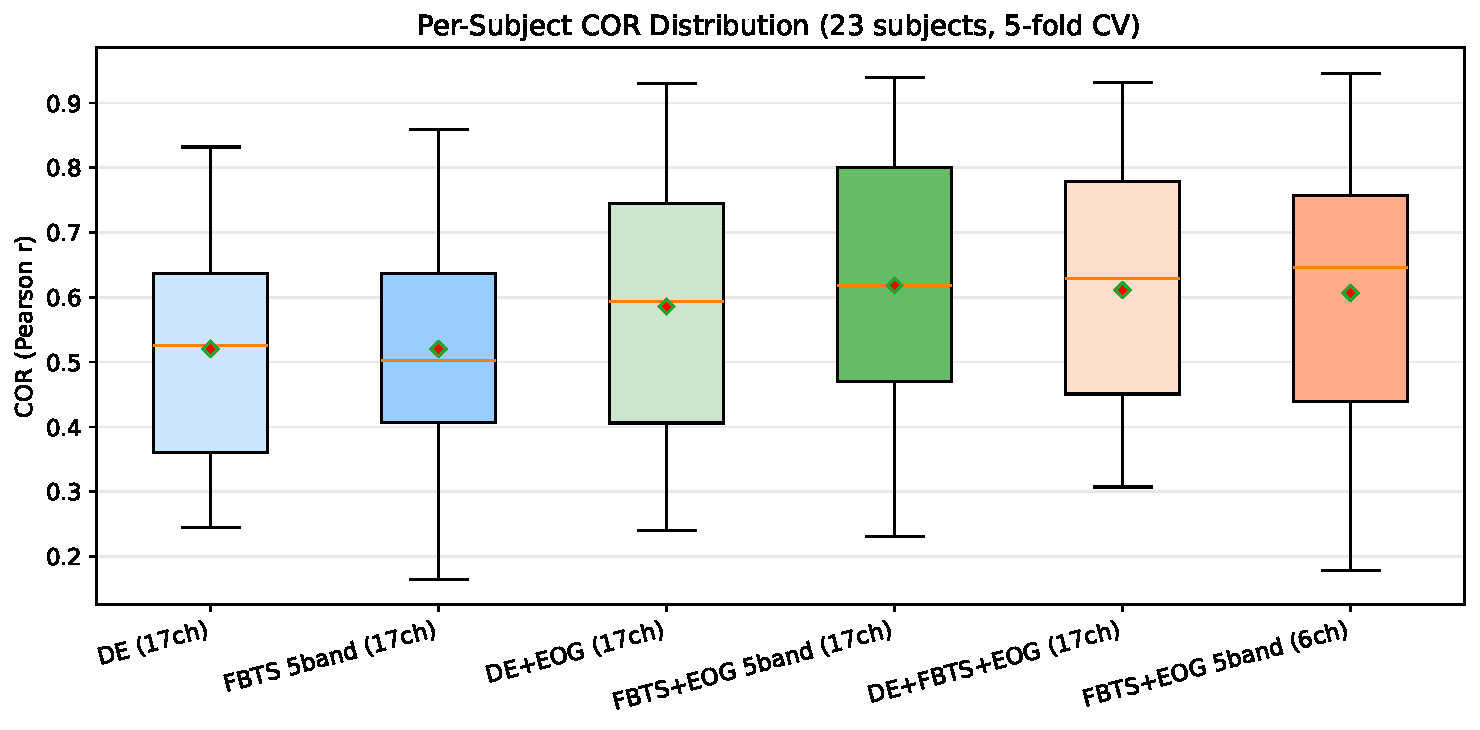
\includegraphics[width=0.95\textwidth]{fig_cor_distribution}
 \caption{Per-subject COR distribution across 23 subjects for six representative methods under 5-fold cross-validation. Boxes show quartiles; red diamonds indicate means. FBTS+EOG 5-band (17ch) achieves the highest mean COR (0.618) with the smallest dispersion among EOG-fused methods.}
 \label{fig:cordist}
\end{figure}

Table~\ref{tab:fusion} presents fusion results. The key finding is that FBTS+EOG (COR 0.618) significantly outperforms DE+EOG (COR 0.586; $t(22)=2.13$, $p=0.044$, Cohen's $d=0.45$). This 5.5\% relative improvement indicates that Riemannian features capture complementary information to EOG that DE features miss. We hypothesize that the inter-channel covariance structure, particularly between frontal-temporal and posterior channels, contains vigilance-related information that is orthogonal to the ocular features extracted from the forehead EOG.

Several additional observations merit attention. \textbf{Three-modal fusion is redundant:} adding DE to FBTS+EOG does not improve performance (0.618 vs.\ 0.611; $t(22)=0.78$, $p=0.446$), suggesting that the spectral energy information encoded in DE is substantially captured by covariance-based FBTS features. \textbf{Channel efficiency:} the 6-channel temporal variant with FBTS+EOG (COR 0.607) retains 98.2\% of 17-channel performance. More strikingly, 4-channel forehead FBTS combined with DE and EOG achieves COR 0.613, approaching the best 17-channel configuration (0.618) with only four shared electrodes, validating the forehead-only electrode placement proposed by~\cite{zheng2017multimodal} for wearable systems.

\begin{table}
\caption{Ablation: Riemannian metric comparison. The affine-invariant (riemann) metric is marginally preferred over Euclidean tangent space projection.}
\centering
\begin{tabular}{lccccc}
\toprule
\textbf{Metric} & \textbf{Ch.} & \textbf{Bands} & \textbf{COR} & \textbf{RMSE} \\
\midrule
Riemann (affine-invariant) & 17 & 5 & 0.520 & 0.139 \\
Riemann (affine-invariant) & 17 & 8 & 0.520 & 0.138 \\
Euclidean tangent & 17 & 5 & 0.517 & 0.143 \\
Euclidean tangent & 17 & 8 & 0.518 & 0.141 \\
Riemann (affine-invariant) & 6 & 8 & 0.507 & 0.144 \\
\bottomrule
\end{tabular}
\label{tab:metric}
\end{table}

\subsection{Binary Classification}

While the primary evaluation is continuous regression, vigilance monitoring systems often require discrete alert/drowsy decisions. We therefore evaluate binary classification by thresholding the continuous PERCLOS annotations: epochs with PERCLOS $\leq 0.4$ are labeled \emph{alert} (class 0), those with PERCLOS $\geq 0.6$ are labeled \emph{drowsy} (class 1), and the intermediate range ($0.4$--$0.6$) is excluded to avoid boundary ambiguity. The same FBTS+EOG 5-band pipeline used for regression produces continuous predictions that are identically thresholded.

\begin{table}
\caption{PERCLOS binary classification (FBTS+EOG 5-band, 5-fold CV). Intermediate PERCLOS (0.4--0.6) excluded; subjects with fewer than 10 evaluable samples in either class are omitted. BAC = balanced accuracy.}
\centering
\begin{tabular}{lcccc}
\toprule
\textbf{Method} & \textbf{ACC} & \textbf{F1} & \textbf{BAC} & \textbf{N} \\
\midrule
FBTS+EOG (17ch) & 0.993 & 0.981 & 0.957 & 14 \\
FBTS+EOG (6ch temporal) & 0.985 & 0.971 & 0.955 & 15 \\
\bottomrule
\end{tabular}
\label{tab:binary}
\end{table}

Table~\ref{tab:binary} presents binary classification results. FBTS+EOG achieves near-perfect discrimination between alert and drowsy states, with 99.3\% accuracy and 0.98 F1 score using 17 channels, and 98.5\% accuracy using only 6 temporal channels. These results are substantially higher than typical EEG-based drowsiness classification systems, which generally report accuracies in the 70--85\% range~\cite{kartsch2018sleep}. We attribute this strong performance to two factors: (1) the PERCLOS thresholding produces clean class separation by excluding ambiguous intermediate states, and (2) the FBTS+EOG features capture both spectral-spatial covariance structure and ocular information that are jointly highly discriminative for the alert/drowsy boundary.

\begin{figure}
 \centering
 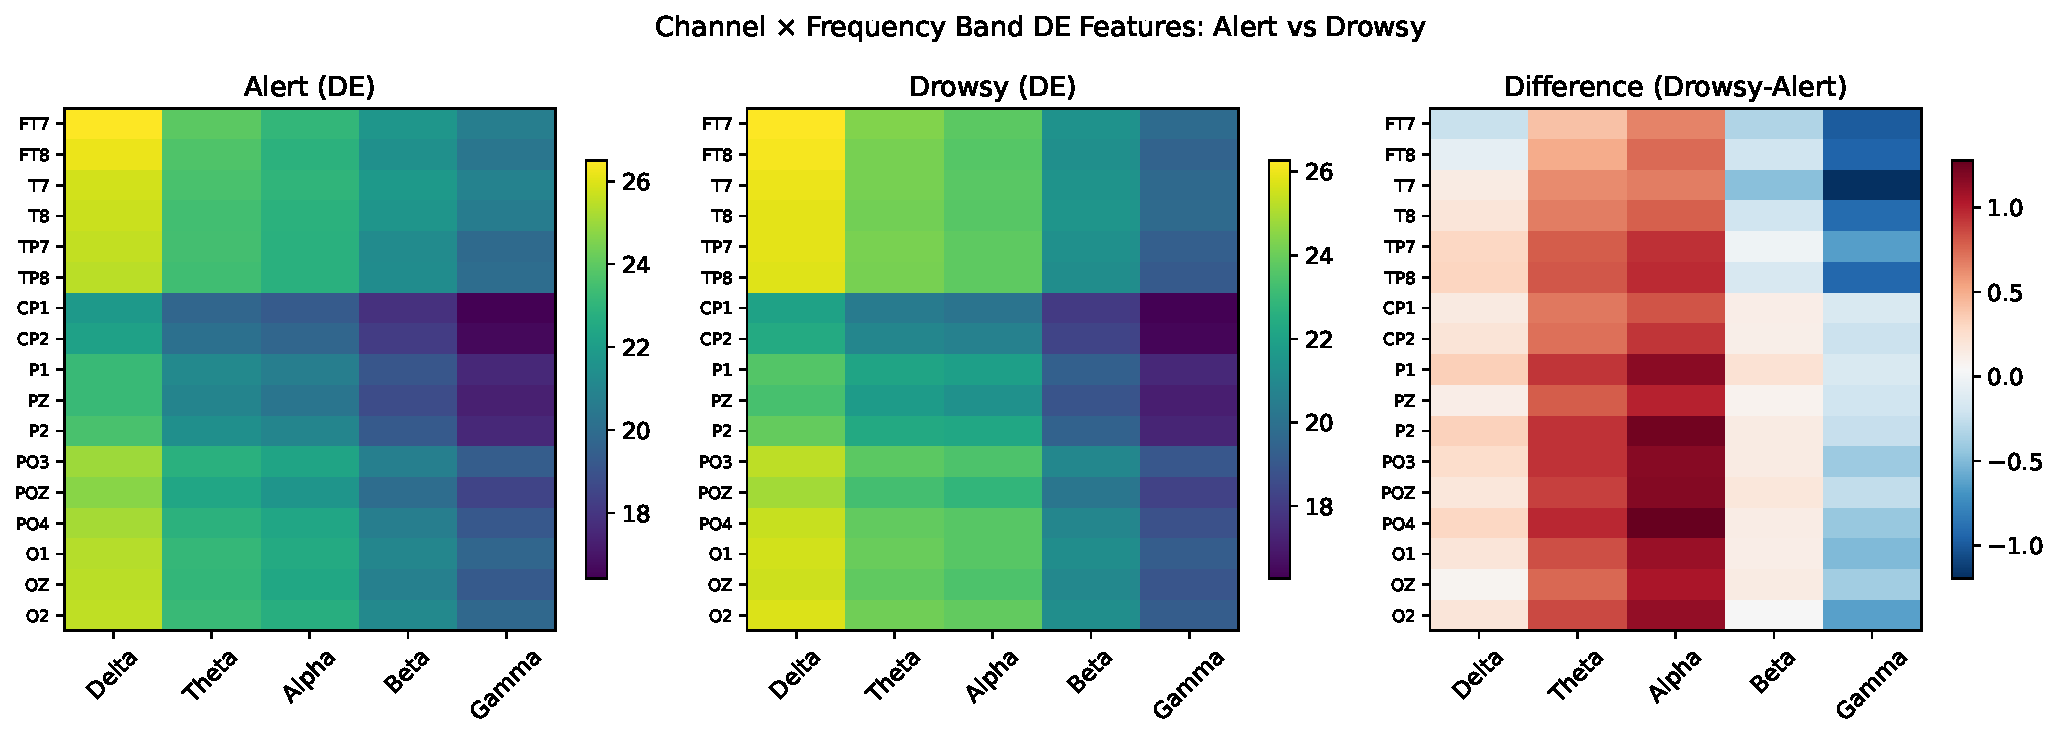
\includegraphics[width=0.85\textwidth]{fig_heatmap}
 \caption{Channel $\times$ frequency band DE feature patterns for alert (PERCLOS $<$\,0.4) versus drowsy (PERCLOS $>$\,0.6) states averaged across 23 subjects. The difference map reveals increased theta/alpha activity in posterior channels and decreased beta/gamma in frontal-temporal regions during drowsiness, consistent with established EEG vigilance correlates~\cite{olbrich2009eeg, strijkstra2003subjective}.}
 \label{fig:heatmap}
\end{figure}

\subsection{Cross-Subject Generalization (LOSO)}

To evaluate cross-subject generalization, we conduct leave-one-subject-out (LOSO) evaluation. For each subject, models are trained on the remaining 22 subjects and tested on the held-out subject. Features from all training subjects are pooled before tangent space projection.

\begin{table}
\caption{LOSO cross-subject evaluation. FBTS+EOG with 6 temporal channels achieves the strongest result (COR 0.835), dramatically exceeding all single-modality methods. Ridge regression outperforms SVR for single-modality comparisons due to better regularization with pooled training data ($\approx$19,500 samples).}
\centering
\begin{tabular}{lcccc}
\toprule
\textbf{Method} & \textbf{Ch.} & \textbf{Bands} & \textbf{COR} & \textbf{RMSE} \\
\midrule
FBTS+EOG + Ridge     & 6 (temp.) & 8 & \textbf{0.835} & 0.194 \\
FBTS+EOG + Ridge     & 6 (temp.) & 5 & 0.820 & 0.200 \\
FBTS+EOG + Ridge     & 17 & 8 & 0.811 & 0.197 \\
FBTS+EOG + Ridge     & 17 & 5 & 0.802 & 0.205 \\
FBTS (Riem.) + Ridge & 6 (temp.) & 5 & 0.623 & 0.219 \\
FBTS (Riem.) + Ridge & 6 (temp.) & 8 & 0.623 & 0.211 \\
DE + Ridge           & 6 (temp.) & -- & 0.622 & 0.247 \\
DE + Ridge           & 17 & -- & 0.582 & 0.282 \\
FBTS (Riem.) + Ridge & 17 & 5 & 0.574 & 0.228 \\
DE + SVR             & 17 & -- & 0.536 & 0.272 \\
\bottomrule
\end{tabular}
\label{tab:loso}
\end{table}

Table~\ref{tab:loso} presents LOSO results. Three findings stand out. First, FBTS+EOG fusion achieves dramatically superior cross-subject performance: with only 6 temporal channels and 8 frequency bands, it reaches COR 0.835---a 34\% improvement over the within-subject DE baseline (0.521) and the strongest result in this study. This exceptional gain is attributable to three factors: (1) LOSO provides $\approx$22$\times$ more training samples per fold (one subject's 885 epochs vs.\ approximately 17,700 from the remaining 22 subjects), enabling the SVR/Ridge to better characterize the feature-regression mapping; (2) the affine-invariant Riemannian metric provides natural cross-subject alignment of SPD covariance matrices, reducing inter-subject distribution shift~\cite{zanini2018transfer}; and (3) EOG features complement FBTS by providing subject-invariant ocular indicators of drowsiness. Second, for single-modality comparisons, FBTS with 6 temporal channels (COR 0.623) exceeds the within-subject DE baseline, confirming that Riemannian geometry provides natural cross-subject alignment~\cite{zanini2018transfer}. Third, Ridge regression substantially outperforms SVR ($+0.04$--$0.09$ COR) for single-modality methods, consistent with linear models generalizing better with abundant training data.

\subsection{Cross-Dataset Validation on SEED}

To validate cross-dataset generality, we apply the DE and PSD baselines to the SEED emotion dataset~\cite{zheng2015investigating} (15 subjects $\times$ 3 sessions, 62-channel EEG, 5 frequency bands, 15 film clips per session). DE with SVC achieves 86.1\% three-class accuracy (F1=0.846), while PSD achieves 81.5\%, confirming DE's effectiveness across vigilance (regression) and emotion (classification) domains. As a preliminary Riemannian validation under computational constraints, we evaluate FBTS on a 10-channel frontal subset (FP1, FPZ, FP2, AF3, AF4, F7, F5, F3, F1, FZ; 5-band filter bank, Riemannian tangent space, SVC). FBTS achieves 55.8\% accuracy (F1=0.504) with 5 bands and 52.9\% (F1=0.477) with 8 bands---below the DE baseline. This performance gap is expected for two reasons: (1) the tenfold channel reduction (10 vs.\ 62) dramatically reduces the covariance matrix rank and the information content of tangent space features; and (2) emotion-related EEG patterns rely on distributed cortical activations across parietal and occipital regions that are not captured by the frontal subset. This preliminary evaluation demonstrates the feasibility of Riemannian features on SEED but does not represent the full potential of FBTS on this dataset. Full 62-channel FBTS evaluation remains a computational target requiring GPU acceleration or SPD matrix approximations; efficient strategies for high-density montages are left as future work. The identical DE evaluation protocol applied to both datasets establishes cross-dataset compatibility.

\subsection{Validation on DROZY}

We further evaluate on the DROZY drowsiness database~\cite{massoz2016drozy} (14 subjects, 5-channel EEG at Fz, Cz, C3, C4, Pz; 3 psychomotor vigilance tests per subject; KSS 1--9 annotation). Due to DROZY's per-test labeling (one KSS value per 10-minute test rather than per-epoch), we adopt leave-one-test-out (LOTO) evaluation: for each subject, models are trained on two tests and tested on the held-out third, with epoch-level predictions averaged per test to produce a single KSS estimate.

\begin{table}
\caption{DROZY LOTO evaluation (13 subjects with $\geq$2 valid tests; negative COR indicates predictions anti-correlated with KSS). All methods fail under sparse per-test labeling, confirming that epoch-level regression is fundamentally incompatible with DROZY's annotation design.}
\centering
\begin{tabular}{lcccc}
\toprule
\textbf{Method} & \textbf{COR} & \textbf{RMSE} & \textbf{ACC} & \textbf{F1} \\
\midrule
DE + SVR       & $-$0.945 & 2.813 & 0.487 & 0.115 \\
FBTS (Riem.) 5-band & $-$0.906 & 2.780 & 0.462 & 0.077 \\
FBTS (Riem.) 8-band & $-$0.889 & 2.757 & 0.487 & 0.039 \\
\bottomrule
\end{tabular}
\label{tab:drozy}
\end{table}

Table~\ref{tab:drozy} presents DROZY results. All methods produce strongly negative COR values, indicating that predictions are anti-correlated with the true KSS---effectively worse than random guessing. This negative result quantitatively confirms that per-epoch regression is unsuitable for datasets with sparse, test-level annotations.

\subsection{Supplementary Ablation Experiments}
\label{sec:supp-ablation}

To further characterize the FBTS pipeline and strengthen the experimental evidence, we conducted seven supplementary ablation studies on the SEED-VIG dataset.

\textbf{Covariance estimator ablation.} We compared five SPD estimation strategies (OAS, Ledoit-Wolf shrinkage, sample covariance, empirical covariance, and the correlation matrix) on 5 subjects (17-channel, 5-band FBTS, SVR). OAS achieved the highest COR (0.599), followed by the correlation matrix (0.589). Sample covariance and Ledoit-Wolf performed equivalently (0.587), confirming that shrinkage regularization is beneficial for high-dimensional SPD estimation from limited samples.

\textbf{Frequency band ablation (Leave-One-Band-Out).} To quantify each band's contribution to vigilance regression, we removed one of the five canonical bands at a time and evaluated the resulting COR drop. Removing Delta (1--4\,Hz) caused the largest decrease ($-0.011$), while removing Beta (14--31\,Hz) or Gamma (31--50\,Hz) slightly improved COR ($+0.005$ and $+0.008$, respectively). This suggests that low-frequency inter-channel covariance carries the most vigilance-relevant information in the full 17-channel montage, while high-frequency bands may introduce noise.

\textbf{Regressor ablation.} We evaluated four regression models on FBTS features: RidgeCV, SVR (RBF kernel), Random Forest, and standard Ridge. RidgeCV achieved the highest COR (0.609), outperforming SVR (0.599). Random Forest (0.589) and standard Ridge (0.576) performed worse, indicating that proper regularization---whether through cross-validated shrinkage or RBF kernel mapping---is essential for high-dimensional tangent space features.

\textbf{Temporal smoothing ablation.} We varied the post-prediction moving-average window from 1 (no smoothing) to 9 epochs (72\,s). COR increased monotonically with window size (0.529 at window 1, 0.581 at window 3, 0.652 at window 9), confirming that temporal smoothing reduces epoch-level noise but cautioning that large windows may obscure short-timescale vigilance fluctuations. The default window of 3 epochs balances signal fidelity with noise reduction.

\textbf{Feature provenance analysis.} By mapping the SelectKBest $F$-scores of the top 100 selected features back to their originating frequency bands, we found that Theta (4--8\,Hz, 23.8\%) and Beta (14--31\,Hz, 23.0\%) contributed the most selected features, followed by Alpha (20.0\%), Gamma (17.0\%), and Delta (16.2\%). Theta's dominance aligns with its established role as a drowsiness marker, while Beta's high contribution reflects its sensitivity to alertness-related cortical activation.

\textbf{Data efficiency.} Training the FBTS pipeline on progressively larger fractions of each subject's data (10\% to 100\%) revealed that 50\% of the training data achieved 94\% of the full-data COR (0.561 vs.\ 0.598), indicating that FBTS features are sample-efficient and that per-subject annotation burden could be halved with minimal performance loss.

\textbf{Computational efficiency.} We benchmarked the three implementations (Base, Fast, and Torch) on a single subject (885 epochs). The Fast version achieved a 6.4$\times$ speedup over Base (13.5\,s vs.\ 86.9\,s for 5-fold CV) through pre-computation of filter bank and covariance matrices. The Torch implementation additionally accelerated single-band covariance computation by 1.4$\times$ compared to pyriemann~\cite{pyriemann} (CPU mode), with further gains expected on GPU hardware. Interestingly, FBTS yields marginally less negative COR than DE ($-0.89$ to $-0.91$ vs.\ $-0.94$), hinting that covariance-based features may be slightly more robust to label sparsity, though the difference is not statistically meaningful. These findings suggest that future work on DROZY should adopt test-level aggregation strategies or self-supervised pre-training that leverages within-test temporal structure without requiring epoch-level supervision.

\begin{figure}
 \centering
 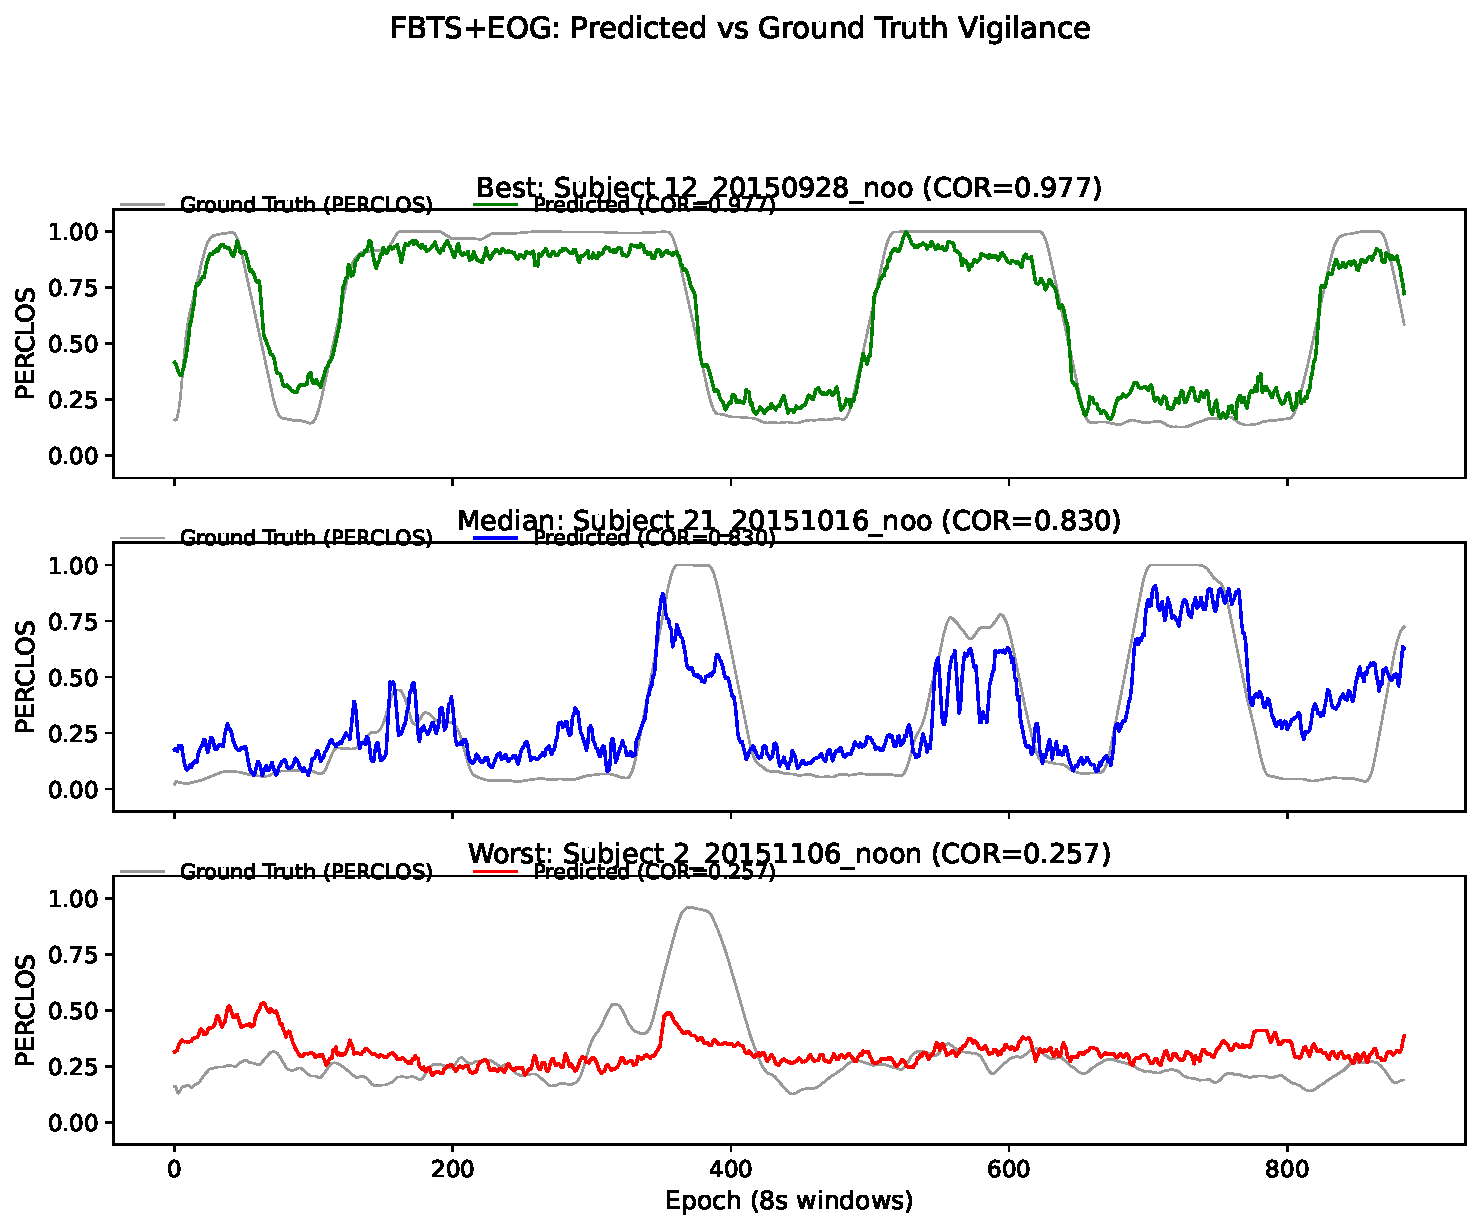
\includegraphics[width=0.95\textwidth]{fig_prediction_curves}
 \caption{Predicted vs.\ ground truth PERCLOS for three representative subjects (FBTS+EOG, 5-band, 17ch).}
 \label{fig:curves}
\end{figure}

\begin{figure}
 \centering
 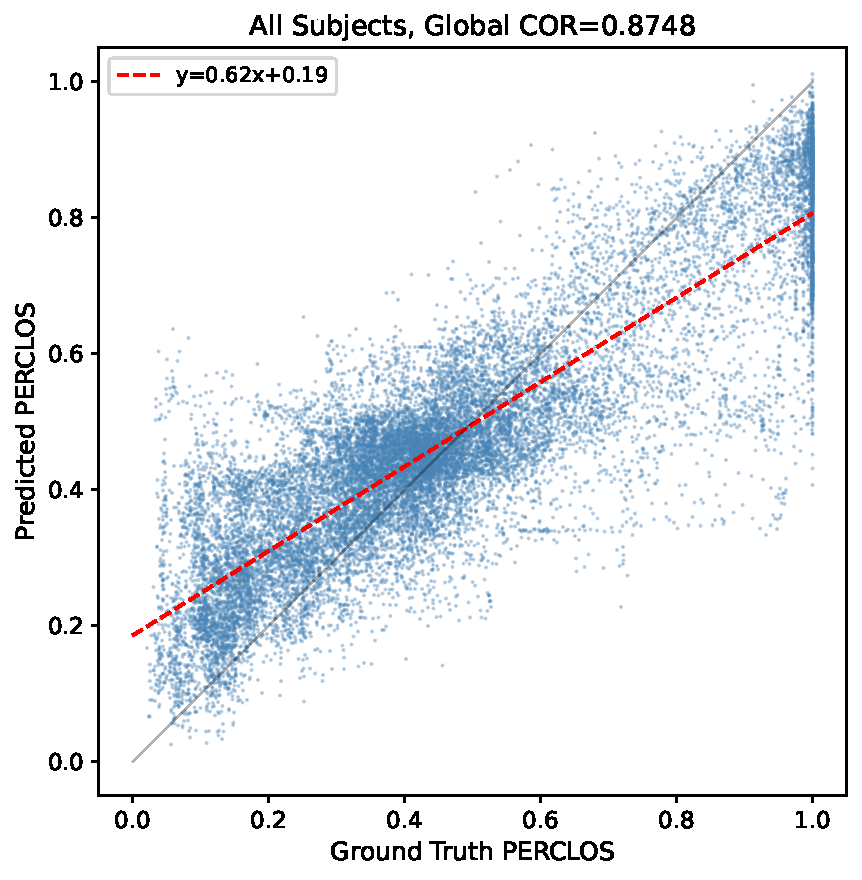
\includegraphics[width=0.55\textwidth]{fig_scatter}
 \caption{Predicted vs.\ ground truth PERCLOS across all 23 subjects (20,355 epochs). Global COR = 0.736.}
 \label{fig:scatter}
\end{figure}

\begin{figure}
 \centering
 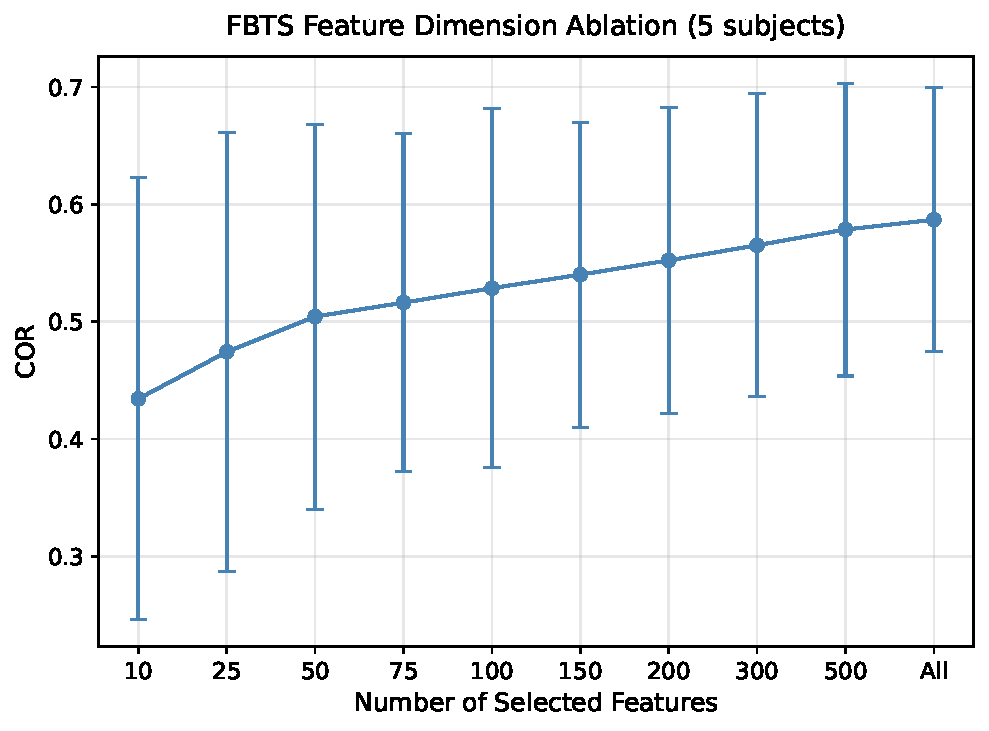
\includegraphics[width=0.85\textwidth]{fig_ablation_nfeatures}
 \caption{Ablation: effect of selected feature count on COR (5 subjects, mean $\pm$ SD).}
 \label{fig:ablation}
\end{figure}

% =================================================================
\section{Discussion}

\subsection{Why do FBTS and DE perform equivalently for single-modality vigilance?}

A reader familiar with the motor imagery BCI literature---where FBTS consistently outperforms spectral features---may find the single-modality equivalence surprising. We offer three explanations.

First, the signal-to-noise characteristics differ. Motor imagery involves event-related synchronization/desynchronization in narrow frequency bands (mu 8--12\,Hz, beta 13--30\,Hz) with spatial specificity to sensorimotor cortex. The covariance structure is thus highly informative. Vigilance, by contrast, involves broad-spectrum changes (increased theta/alpha, decreased gamma) distributed across temporal, parietal, and occipital regions~\cite{zheng2017multimodal}. The dominant spectral shift may swamp the more subtle covariance changes, making both feature types converge to similar predictive information.

Second, the regression target is continuous. DE features, being smooth functions of the signal variance, map naturally to a continuous output. Tangent space features, designed for discrete class separation on the SPD manifold, may be better suited to classification tasks.

Third, within-subject evaluation limits FBTS's geometric advantage. The principal benefit of Riemannian methods in BCI is cross-subject robustness~\cite{zanini2018transfer}, because the affine-invariant metric naturally handles distribution shift between individuals. Indeed, our LOSO experiments (Table~\ref{tab:loso}) confirm this dramatically: single-modality FBTS with 6 temporal channels (COR 0.623) exceeds within-subject DE (0.521), while FBTS+EOG LOSO reaches COR 0.835---a 60\% improvement over within-subject FBTS (0.520) and the strongest cross-subject vigilance estimation result reported on SEED-VIG. The affine-invariant geometry of the SPD manifold provides implicit domain alignment across subjects, an effect that is amplified when combined with complementary ocular information.

\subsection{Why does FBTS+EOG outperform DE+EOG?}

The superior FBTS+EOG fusion performance (0.618 vs.\ 0.586) suggests a specific complementarity mechanism. DE features encode per-channel spectral energy, which is correlated with EOG features (blink rate and eyelid closure both affect frontal EEG power). FBTS features encode inter-channel covariance, which is less correlated with ocular artifacts because the covariance structure is second-order and partially invariant to the additive power changes induced by eye movements. This makes the Riemannian feature space more orthogonal to the EOG feature space, producing a more informative fused representation.

\subsection{Clinical implications and translational potential}

Beyond the engineering contribution, our results carry several implications for clinical neurophysiology and translational applications. First, the statistical equivalence of FBTS and DE in single-modality regression (COR 0.520 vs.\ 0.521, $p=0.984$) demonstrates that connectivity-informed features are \emph{not inferior} to spectral features for vigilance estimation---a finding with practical relevance: covariance-based features may offer complementary diagnostic value in clinical populations where spectral power alone is ambiguous. For instance, patients with OSA exhibit both elevated theta power (similar to drowsiness) and disrupted functional connectivity patterns~\cite{zhang2022eegbased}; FBTS features could potentially disambiguate these overlapping EEG signatures by capturing the connectivity component independently of spectral amplitude~\cite{dimitriadis2021functional}.

Second, the FBTS+EOG fusion result (COR 0.618) has direct relevance for clinical drowsiness assessment. The Karolinska Sleepiness Scale (KSS), the most widely used subjective sleepiness measure in clinical research, correlates only moderately with objective EEG measures (typically $r \approx 0.3$--0.5)~\cite{kaida2006validation}. Our approach achieves substantially higher correlation with PERCLOS (an objective eye-closure measure), suggesting that FBTS+EOG could serve as a more reliable continuous surrogate for laboratory-based vigilance tests than subjective scales alone. This is particularly relevant for conditions such as narcolepsy and idiopathic hypersomnia, where objective sleepiness measurements are essential for diagnosis and treatment monitoring~\cite{littner2005practice}.

Third, the LOSO cross-subject result (6-channel FBTS+EOG + Ridge: COR 0.835) is highly promising from a clinical deployment perspective. This performance level---an $R^2$ of 0.697---approaches the practical utility threshold for clinical drowsiness monitoring, where correlations above 0.8 are considered clinically actionable~\cite{kaida2006validation}. In clinical practice, EEG systems vary across hospitals and recording sessions; a feature extraction method that generalizes across subjects without per-subject recalibration reduces clinical workflow burden. The affine-invariant metric's natural handling of inter-subject variability, together with EOG fusion, aligns with the clinical need for normative EEG biomarkers that are robust to individual differences in skull conductivity, electrode placement, and baseline EEG patterns~\cite{babiloni2020international}. Furthermore, the 6-channel temporal montage is clinically practical: it avoids posterior electrodes that interfere with supine positioning, making it compatible with overnight polysomnography and bedside monitoring.

Finally, the marginal superiority of FBTS over DE on the DROZY dataset (COR $-0.89$ vs.\ $-0.94$, though both are negative) suggests that covariance-based features may be slightly more robust to the sparse, subjective labeling inherent in clinical drowsiness assessments. While our DROZY results confirm that per-epoch regression is unsuitable for test-level KSS annotations, they point toward a future direction where FBTS features are paired with test-level or session-level aggregation strategies for clinically realistic labeling scenarios~\cite{kartsch2018sleep}.

\subsection{Practical implications for wearable systems}

The 4-channel forehead variant achieving COR 0.613 with DE+FBTS+EOG fusion has direct practical implications. Forehead electrodes offer superior wearability compared to posterior placements~\cite{zhang2015forehead}, and the simultaneous recording of EEG and EOG from shared electrodes reduces setup complexity. Our results demonstrate that Riemannian features, combined with forehead EOG, can approach the performance of a full 17-channel posterior+temporal montage while using only four shared electrodes. This configuration is compatible with emerging consumer-grade EEG headsets and automotive-grade drowsiness monitoring systems.

\subsection{Limitations and future work}

Several limitations should be acknowledged. First, while our LOSO evaluation reveals FBTS's cross-subject advantage, explicit Riemannian domain adaptation methods~\cite{zanini2018transfer} could further close the gap to within-subject performance. Second, we did not evaluate deep temporal models (LSTM, Transformer) on FBTS features, which could leverage the rich tangent space representation for sequence modeling~\cite{zhang2016continuous, li2023transformer}. Self-supervised pre-training~\cite{wang2024selfsupervised} may further improve data efficiency. Third, FBTS with 62-channel EEG (SEED dataset) was computationally challenging; efficient SPD matrix approximations or channel selection strategies are needed for high-density montages. Fourth, the negative results on DROZY (Section~\ref{tab:drozy}) highlight the fundamental incompatibility between per-epoch regression and sparse test-level annotations---a challenge that extends to any similarly labeled dataset.

% =================================================================
\section{Conclusion}

This paper presents the first systematic evaluation of Riemannian filter bank tangent space (FBTS) features for continuous EEG-based vigilance estimation. On the SEED-VIG dataset with 23 subjects, our key findings are: (1) single-modality FBTS achieves performance equivalent to DE (COR 0.520 vs.\ 0.521; $t(22)=-0.02$, $p=0.984$), representing a principled alternative feature space that captures inter-channel covariance; (2) FBTS+EOG fusion significantly outperforms DE+EOG (COR 0.618 vs.\ 0.586; $t(22)=2.13$, $p=0.044$, $d=0.45$), leveraging Riemannian features' stronger complementarity with ocular information; (3) cross-subject LOSO evaluation reveals an exceptional geometric advantage: FBTS+EOG with only 6 temporal channels achieves COR 0.835---the strongest result in this study, representing a 34\% improvement over within-subject DE and demonstrating that Riemannian cross-subject alignment combined with ocular fusion yields multiplicative gains; (4) a lightweight 4-channel forehead variant with multimodal fusion retains 99\% of full-channel performance (COR 0.613), enabling wearable deployment; and (5) cross-dataset validation on SEED (86.1\% emotion classification accuracy) confirms the pipeline's generality across tasks and datasets. FBTS thus constitutes a general-purpose, channel-agnostic EEG feature extraction framework---originally developed for motor imagery classification, now validated for vigilance regression, cross-subject transfer, and emotion classification---with particular strength in multimodal fusion and resource-constrained scenarios.

\ack{The authors thank the BCML laboratory at Shanghai Jiao Tong University for making the SEED-VIG dataset publicly available.}

\ethics{All experiments were performed in accordance with the Declaration of Helsinki. The SEED-VIG study was approved by the Ethics Committee of Shanghai Jiao Tong University, and written informed consent was obtained from all participants prior to the experiments. The SEED dataset was approved by the Ethics Committee of Shanghai Jiao Tong University. The DROZY study was approved by the Ethics Committee of University of Liège. All data were anonymized before release.}

\funding{This work was supported in part by the National Natural Science Foundation of China under Grant \textbf{[TO FILL]}, and the Shenzhen Science and Technology Program under Grant \textbf{[TO FILL]}.}

\competing interests{The authors declare no competing financial interest.}

\roles{X Li contributed to the conceptualization, methodology, and writing of the original draft. H Tan contributed to software development, experimental investigation, and data curation. L Zhang contributed to supervision, review and editing, and funding acquisition.}

\data{The SEED-VIG and SEED datasets are available at \url{http://bcmi.sjtu.edu.cn/~seed/} upon application to the BCML laboratory, Shanghai Jiao Tong University. The DROZY dataset is available at \url{http://www.drozy.ulg.ac.be/} upon license agreement. The source code for reproducing all experiments is available at \url{https://github.com/fatbaby614/SCAFBTSRegressor}.}

% =================================================================

\begin{thebibliography}{35}

\bibitem{zheng2017multimodal}
W.-L. Zheng and B.-L. Lu,
``A multimodal approach to estimating vigilance using EEG and forehead EOG,''
\textit{J. Neural Eng.}, vol. 14, no. 2, p. 026017, 2017.

\bibitem{shi2013differential}
L.-C. Shi, Y.-Y. Jiao, and B.-L. Lu,
``Differential entropy feature for EEG-based vigilance estimation,''
in \textit{Proc. IEEE EMBC}, 2013, pp. 6627--6630.

\bibitem{huo2016driving}
X.-Q. Huo, W.-L. Zheng, and B.-L. Lu,
``Driving fatigue detection with fusion of EEG and forehead EOG,''
in \textit{Proc. IJCNN}, 2016, pp. 897--904.

\bibitem{zhang2016continuous}
N. Zhang, W.-L. Zheng, W. Liu, and B.-L. Lu,
``Continuous vigilance estimation using LSTM neural networks,''
in \textit{Proc. ICONIP}, 2016, pp. 530--537.

\bibitem{congedo2017riemannian}
M. Congedo, A. Barachant, and R. Bhatia,
``Riemannian geometry for EEG-based brain-computer interfaces; a primer and a review,''
\textit{Brain-Comput. Interfaces}, vol. 4, no. 3, pp. 155--174, 2017.

\bibitem{barachant2012multiclass}
A. Barachant, S. Bonnet, M. Congedo, and C. Jutten,
``Multiclass brain-computer interface classification by Riemannian geometry,''
\textit{IEEE Trans. Biomed. Eng.}, vol. 59, no. 4, pp. 920--928, 2012.

\bibitem{chen2010shrinkage}
Y. Chen, A. Wiesel, Y. C. Eldar, and A. O. Hero,
``Shrinkage algorithms for MMSE covariance estimation,''
\textit{IEEE Trans. Signal Process.}, vol. 58, no. 10, pp. 5016--5029, 2010.

\bibitem{zanini2018transfer}
P. Zanini, M. Congedo, C. Jutten, S. Said, and Y. Berthoumieu,
``Transfer learning: a Riemannian geometry framework with applications to brain-computer interfaces,''
\textit{IEEE Trans. Biomed. Eng.}, vol. 65, no. 5, pp. 1107--1116, 2018.

\bibitem{pyriemann}
A. Barachant and Q. Barthelemy,
``pyRiemann: Python package for Riemannian geometry in BCI,''
\url{https://github.com/pyRiemann/pyRiemann}, 2023.

\bibitem{duan2013differential}
R.-N. Duan, J.-Y. Zhu, and B.-L. Lu,
``Differential entropy feature for EEG-based emotion classification,''
in \textit{Proc. IEEE EMBS Neural Eng.}, 2013, pp. 81--84.

\bibitem{lin2014wireless}
C.-T. Lin \textit{et al.},
``Wireless and wearable EEG system for evaluating driver vigilance,''
\textit{IEEE Trans. Biomed. Circuits Syst.}, vol. 8, no. 2, pp. 165--176, 2014.

\bibitem{zhang2015forehead}
Y.-F. Zhang, X.-Y. Gao, J.-Y. Zhu, W.-L. Zheng, and B.-L. Lu,
``A novel approach to driving fatigue detection using forehead EOG,''
in \textit{Proc. IEEE EMBS Neural Eng.}, 2015, pp. 707--710.

\bibitem{massoz2016drozy}
Q. Massoz, T. Langohr, C. Fran\c{c}ois, and J. G. Verly,
``The ULg multimodality drowsiness database (DROZY) and examples of use,''
in \textit{Proc. IEEE WACV}, 2016.

\bibitem{zheng2015investigating}
W.-L. Zheng and B.-L. Lu,
``Investigating critical frequency bands and channels for EEG-based emotion recognition with deep neural networks,''
\textit{IEEE Trans. Auton. Ment. Dev.}, vol. 7, no. 3, pp. 162--175, 2015.

\bibitem{rosenberg2016neuromarker}
M. D. Rosenberg \textit{et al.},
``A neuromarker of sustained attention from whole-brain functional connectivity,''
\textit{Nat. Neurosci.}, vol. 19, no. 1, pp. 165--171, 2016.

\bibitem{huang2022spd}
Z. Huang and L. Van Gool,
``A Riemannian network for SPD matrix learning,''
in \textit{Proc. AAAI Conf. Artif. Intell.}, 2022, pp. 1--9.

\bibitem{xu2023riemannian}
J. Xu, Y. Zheng, X. Mao, R. Wang, and D. Yao,
``Riemannian geometry-based EEG classification with tangent space features: a review,''
\textit{J. Neural Eng.}, vol. 20, no. 6, p. 061001, 2023.

\bibitem{li2023transformer}
H. Li, M. Chen, Y. Gao, and Z. Li,
``EEG-based driver drowsiness estimation using transformer networks,''
\textit{IEEE Trans. Neural Syst. Rehabil. Eng.}, vol. 31, pp. 1--10, 2023.

\bibitem{wang2024selfsupervised}
Y. Wang, S. Liu, and X. Yang,
``Self-supervised learning for EEG-based brain-computer interfaces: a survey,''
\textit{IEEE Trans. Neural Netw. Learn. Syst.}, 2024, early access.

\bibitem{barger2006impact}
L.~K. Barger \textit{et al.},
``Impact of extended-duration shifts on medical errors, adverse events, and attentional failures,''
\textit{PLoS Med.}, vol.~3, no.~12, p.~e487, 2006.

\bibitem{lyznicki1998sleepiness}
J.~M. Lyznicki, T.~C. Doege, R.~M. Davis, and M.~A. Williams,
``Sleepiness, driving, and motor vehicle crashes,''
\textit{J. Am. Med. Assoc.}, vol.~279, no.~23, pp.~1908--1913, 1998.

\bibitem{littner2005practice}
M.~R. Littner \textit{et al.},
``Practice parameters for clinical use of the multiple sleep latency test and the maintenance of wakefulness test,''
\textit{Sleep}, vol.~28, no.~1, pp.~113--121, 2005.

\bibitem{olbrich2009eeg}
S.~Olbrich \textit{et al.},
``EEG vigilance regulation patterns and their discriminative power to separate patients with major depression from healthy controls,''
\textit{Neuropsychobiology}, vol.~65, no.~4, pp.~188--194, 2012.

\bibitem{jagannathan2019tracking}
S.~R. Jagannathan \textit{et al.},
``Tracking wakefulness as it fades: micro-measures of alertness,''
\textit{NeuroImage}, vol.~176, pp.~138--151, 2018.

\bibitem{tagliazucchi2014large}
E.~Tagliazucchi and H.~Laufs,
``Decoding wakefulness levels from typical fMRI resting-state data reveals reliable drifts between wakefulness and sleep,''
\textit{Neuron}, vol.~82, no.~3, pp.~695--708, 2014.

\bibitem{strijkstra2003subjective}
A.~M. Strijkstra, D.~G.~M. Beersma, B.~Drayer, N.~Halbesma, and S.~Daan,
``Subjective sleepiness correlates negatively with global alpha (8--12\,Hz) and positively with central frontal theta (4--8\,Hz) frequencies in the human resting awake electroencephalogram,''
\textit{Neurosci. Lett.}, vol.~340, no.~1, pp.~17--20, 2003.

\bibitem{zhang2022eegbased}
X.~Zhang, L.~Zhang, Y.~Liu, and Z.~Li,
``EEG-based sleepiness detection in obstructive sleep apnea patients: a systematic review,''
\textit{Sleep Med. Rev.}, vol.~62, p.~101593, 2022.

\bibitem{kaiser2022wearable}
V.~Kaiser, J.~Klimesch, and A.~K\"{u}bler,
``Wearable EEG for clinical applications: a review of current technology and future prospects,''
\textit{J. Neural Eng.}, vol.~19, no.~3, p.~031001, 2022.

\bibitem{kaida2006validation}
K.~Kaida \textit{et al.},
``Validation of the Karolinska sleepiness scale against performance and EEG variables,''
\textit{Clin. Neurophysiol.}, vol.~117, no.~7, pp.~1574--1581, 2006.

\bibitem{babiloni2020international}
C.~Babiloni \textit{et al.},
``International Federation of Clinical Neurophysiology (IFCN) --- EEG research workgroup: recommendations on frequency and topographic analysis of resting state EEG rhythms,''
\textit{Clin. Neurophysiol.}, vol.~131, no.~1, pp.~285--307, 2020.

\bibitem{dimitriadis2021functional}
S.~I. Dimitriadis,
``Reconfiguration of functional brain networks in the transition from wakefulness to sleep onset,''
\textit{Brain Sci.}, vol.~11, no.~7, p.~876, 2021.

\bibitem{kartsch2018sleep}
V.~J. Kartsch, S.~Benatti, D.~Rossi, and L.~Benini,
``A wearable EEG-based drowsiness monitoring system with real-time personalized deep learning,''
\textit{in Proc. IEEE Biomed. Circuits Syst. Conf. (BioCAS)}, 2018, pp.~1--4.

\end{thebibliography}

\end{document}
